\documentclass[%
11pt,%
%oneside,%
twoside,%
%twocolumn,%
titlepage,%
%fleqn,%
a4page,%
german,%
headsepline%
]{scrartcl}

%\usepackage{fancyhdr}
\usepackage{scrpage2}
\usepackage{lastpage}
\usepackage{geometry}
\usepackage{graphicx}
\usepackage[utf8]{inputenc}
\usepackage[ngerman]{babel}
\usepackage{lscape}
\usepackage{mymath}
\usepackage{units}
\usepackage{nicefrac}
\usepackage{pgf,tikz}
\usetikzlibrary{arrows}
\usepackage{colortbl}
\usepackage{hhline}
\usepackage{multirow}
\usepackage[extendedchars]{grffile}
\usepackage{caption}
\usepackage{multicol,calc}
\usepackage{blindtext}
\usepackage{pdfpages}
\usepackage{hyperref}
\usepackage[official]{eurosym}
\usepackage{framed}
\usetikzlibrary{arrows}
\usetikzlibrary{positioning}
\usetikzlibrary{shadows}

%\usepackage{romannum}
\usepackage{longtable}
\usepackage{listings}
\usepackage{wrapfig}


% Command, um Tabellen-Spalten anzupassen
\newcommand{\spaltenheight}{\rule{0mm}{3ex}}
\newcommand{\spaltenwidth}{\rule{3cm}{0mm}}
\newcommand{\spaltensep}{\\[1ex]}
%\arrayrulecolor{darkgreen}
\doublerulesepcolor{white}
\definecolor{lightyellow}{rgb}{1,1,0.8}
\definecolor{Gray}{gray}{0.9}


% Pagestyle/Layout
%\geometry{a4paper , tmargin =2.5cm,	bmargin=3cm, lmargin =2.5cm,	rmargin =2.5cm,	headheight=3em, headsep=1em, footskip=1cm}
\setlength{\parindent}{0pt} \setlength{\parskip}{1em}
%für TwoSide
\lehead{\headmark\pagemark}
%\cehead{}
%\rehead{}
%\lohead{}
%\cohead{}
%\rohead{\headmark}
%für OneSide
%\ihead{}
%\chead{}
%\ohead{}
\setheadsepline{0.5pt} % Linie zur Begrenzung
\setfootsepline{0.5pt} % Linie zur Begrenzung
\pagestyle{headings} % gemachte Einstellungen anwenden


\subject{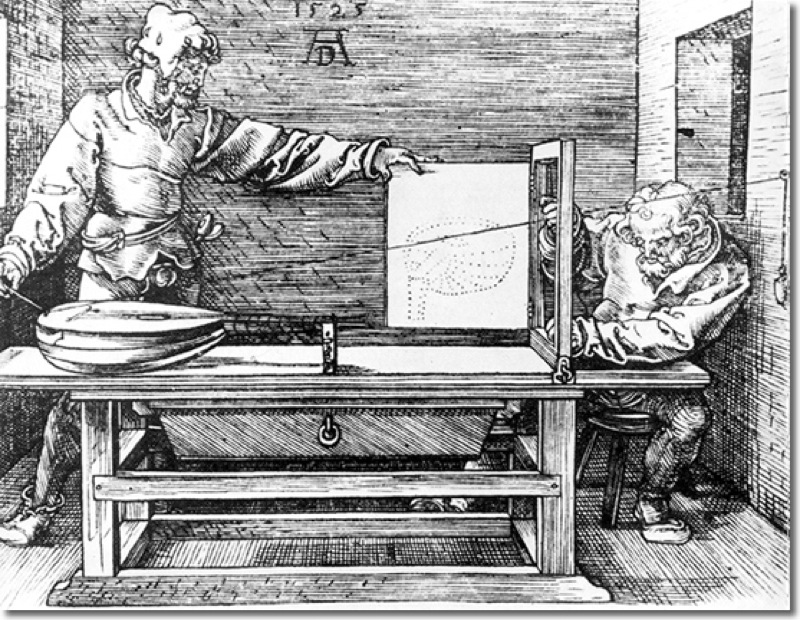
\includegraphics[width=0.618\textwidth]{pictures/durer}}
\title{Stereometrie}
\subtitle{3D}
\author{}
\date{}
%\lowertitleback{
%\includegraphics[height=1.1cm]{/Users/jormawassmer/Pictures/logokoeniz.jpg}%
%\copyright Jorma Wassmer
%1. Auflage, Februar 2011
%}


\begin{document}
\maketitle
\tableofcontents
%\thispagestyle{empty}
\cleardoublepage
%\setcounter{page}{1}

\section{R\"aumliche Geometrie}
\subsection{Die Raumelemente}
\begin{bem}
F\"arben Sie in den folgenden Figuren und Ihren Skizzen, soweit sinnvoll, die Geraden und Ebenen jeweils mit verschiedenen Farben.
\end{bem}
\subsubsection{Punkt, Gerade, Ebene}
\begin{center}
\definecolor{zzttqq}{rgb}{0.6,0.2,0}
\definecolor{qqqqff}{rgb}{0,0,1}
\begin{tikzpicture}[line cap=round,line join=round,>=triangle 45,x=0.5cm,y=0.5cm]
\clip(-2.12,-1.12) rectangle (14.58,5.28);
\fill[color=zzttqq,fill=zzttqq,fill opacity=0.1] (13,4.44) -- (8.04,4.44) -- (4.64,1) -- (10.62,1) -- cycle;
\draw [domain=-2.12:14.58] plot(\x,{(-2.71--4.24*\x)/4.22});
\draw [color=zzttqq] (13,4.44)-- (8.04,4.44);
\draw [color=zzttqq] (8.04,4.44)-- (4.64,1);
\draw [color=zzttqq] (4.64,1)-- (10.62,1);
\fill [color=qqqqff] (-0.74,2.92) circle (1.5pt);
\draw[color=qqqqff] (-1,3.3) node {$P$};
\draw[color=black] (0.22,0.32) node {$g$};
\draw[color=zzttqq] (5.7,1.5) node {$E$};
\end{tikzpicture}
\end{center}

Eine Gerade ist eindeutig durch zwei Punkte bestimmt. Man schreibt etwa $g=(A,B)$ f\"ur diejenige Gerade, welche durch die Punkte A und B geht.

\begin{ueb} \ \\[-4ex]
\begin{enumeratea}
\item Von den Punkten A, B, C, D liegen die ersten drei auf einer Geraden. Wie viele Geraden sind durch diese Punkte bestimmt?
\item Wie viele Geraden sind durch die Eckpunkte eines W\"urfels bestimmt?
\item Wie viele Geraden sind durch $n$ Punkte in allgemeiner Lage bestimmt?
\end{enumeratea}
\end{ueb}

\noindent Eine Ebene ist eindeutig bestimmt durch:
\begin{itemize}
\item drei Punkte, die nicht auf einer Geraden liegen (drei nicht kollineare Punkte)
\item eine Gerade und ein Punkte, der nicht auf ihr liegt
\item zwei sich schneidende Geraden
\item zwei parallele Geraden, die keinen gemeinsamen Punkt haben
\end{itemize}

\begin{ueb} \ \\[-4ex]
\begin{enumeratea}
\item Von $6$ Punkten liegen genau $5$ in einer Ebene. Wie viele Ebenen sind durch diese $6$ Punkte bestimmt?
\item Wie viele Ebenen sind durch die $8$ Eckpunkte eines W\"urfels bestimmt? Wie viele dieser Ebenen enthalten genau $4$, wie viele genau $3$ Eckpunkte?
\item Wie viele Ebenen sind durch $n$ Punkte in allgemeiner Lage bestimmt?
\item Wie viele Ebenen sind durch $n$ parallele Geraden im Raum im allgemeinen bestimmt?
\end{enumeratea}
\end{ueb}

\begin{ueb}
Gegeben ist ein Punkt P auf einer Geraden g im Raum. Ist die zu g senkrechte Gerade durch P eindeutig bestimmt?
\end{ueb}

\subsubsection{Gerade und Gerade}
F\"ur die gegenseitige Lage zweier Geraden g und h im Raum sind vier F\"alle zu unterscheiden:
\begin{itemize}
\item g und h haben keinen Punkt gemeinsam, und es gibt eine Ebene, in der sie beide enthalten sind; g und h sind parallel, $g\cap h=\emptyset$.
\item g und h haben alle Punkte gemeinsam, d.h., sie sind identisch, $g=h$.
\item g und h haben genau einen Punkt gemeinsam, d.h., g und h schneiden sich, $g\cap h=\{S\}$.
\item g und h haben keinen gemeinsamen Punkt, und sie sind in keiner gemeinsamen Ebene enthalten, d.h., g und h sind zueinander windschief.
\end{itemize}

\begin{ueb}
Verbinden Sie vier nicht in einer Ebene liegende Punkte zu einem Viereck. Was l\"asst sich \"uber die Diagonalen sagen?
\end{ueb}
\begin{ueb}
Die Geraden g und h seien mit der Geraden s windschief. Sind dann g und h windschief?
\end{ueb}

\subsubsection{Gerade und Ebene}
F\"ur die gegenseitige Lage einer Geraden g und einer Ebene E sind drei F\"alle zu unterscheiden:
\begin{itemize}
\item g und E haben keinen gemeinsamen Schnittpunkt, d.h., g ist parallel zu E, $g\cap E=\emptyset$.
\item alle Punkte von g liegen in E, d.h., g liegt in E, g ist parallel zu E.
\item g und E haben genau einen gemeinsamen Punkt, d.h., g schneidet die Ebene E (Durchstosspunkt D), $g\cap E=\{D\}$
\end{itemize}

\begin{ueb}
g und h seien zwei zu einer Ebene E parallele Geraden. Welche Aussagen sind richtig:
\begin{enumeratea}
\item $g\| h$
\item $g\bot h$
\item $g\cap h=\emptyset$
\item g und h sind windschief
\item es l\"asst sich keine Aussage machen
\end{enumeratea}
\end{ueb}

\begin{ueb}
Die Ebenen $E_1$ und $E_2$ seien parallel ohne gemeinsamen Punkt. Wie liegt die Gerade $r$ zu $E_2$, wenn $r$
\begin{enumeratea}
\item parallel zu $E_1$ ist
\item $E_1$ schneidet
\item in $E_1$ liegt?
\end{enumeratea}
\end{ueb}

\subsubsection{Ebene und Ebene}
F\"ur die gegenseitige Lage zweier Ebenen $E_1$ und $E_2$ sind drei F\"alle zu unterscheiden.
\begin{itemize}
\item $E_1$ und $E_2$ haben keinen gemeinsamen Punkt; sie sind parallel, $E_1\cap E_2=\emptyset$.
\item $E_1$ und $E_2$ haben alle Punkte gemeinsam, d.h., sie sind identisch; $E_1=E_2$.
\item $E_1$ und $E_2$ haben eine Gerade gemeinsam, d.h. sie schneiden sich (Schnittgerade $s$); $E_1\cap E_2=\{s\}$
\end{itemize}

\begin{ueb}
Wie viele Schnittgeraden ergeben sich durch $n$ Ebenen in allgemeiner Lage?
\end{ueb}
\begin{ueb}
g und h seien windschiefe Geraden. Die Gerade s schneidet sowohl g als auch h. Wie viele Ebenen sind durch diese drei Geraden bestimmt?
\end{ueb}
\begin{ueb}
Die Geraden r und s seien windschief. R ist ein Punkt auf r, S ein Punkt auf s. Welches ist die Schnittgerade der Ebenen $E_1=(R,s)$ und $E_2=(S,r)$?
\end{ueb}

\begin{ueb}
Auf die Seiten eines W\"urfels wurden die Ziffern 1 bis 6 willk\"urlich verteilt. Kann man aus den beiden Ansichten des W\"urfels erkennen, welche Ziffer sich gegen\"uber der 1 befindet?
\begin{center}
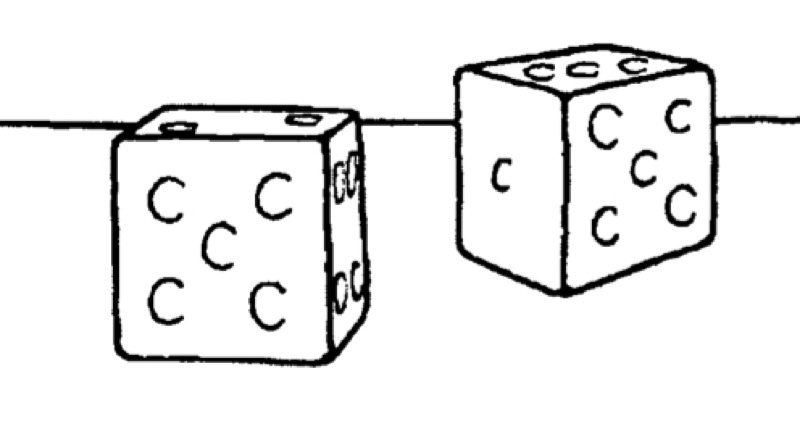
\includegraphics[width=7cm]{pictures/wuerfel}
\end{center}
\end{ueb}

\begin{ueb}
Kippe den W\"urfel aus dem mittleren Feld auf- oder abw\"arts, nach links oder rechts, jedoch nie diagonal. Nach sechs Kippbewegungen soll der W\"urfel mit der Augenzahl 6 nach oben auf dem Feld 1 liegen. Ist das mšglich?
\begin{center}
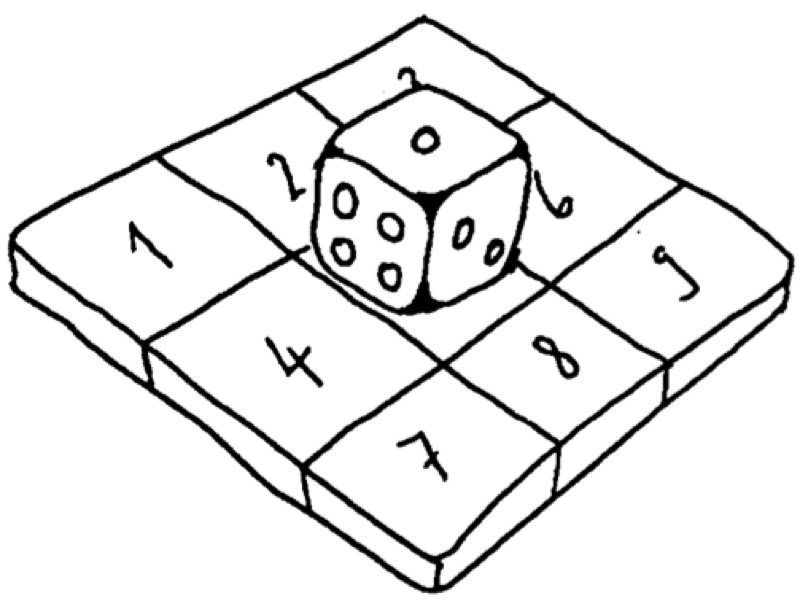
\includegraphics[width=7cm]{pictures/wuerfelfeld}
\end{center}
\end{ueb}

\pagebreak

\subsection{Die Parallelprojektion}
\begin{defn}
Durch den Punkt $P$ wird ein Projektionsstrahl parallel zur Projektionsrichtung $r$ gelegt. Den Durchstosspunkt $P'$ mit der Bildebene nennt man das Bild oder die\textbf{Projektion} von $P$.
\end{defn}
\begin{center}
\definecolor{zzttqq}{rgb}{0.6,0.2,0}
\definecolor{xdxdff}{rgb}{0.49,0.49,1}
\definecolor{qqqqff}{rgb}{0,0,1}
\begin{tikzpicture}[line cap=round,line join=round,>=triangle 45,x=0.5cm,y=0.5cm]
\clip(-4.3,-1.06) rectangle (8.46,6.3);
\fill[color=zzttqq,fill=zzttqq,fill opacity=0.1] (6.12,0) -- (-4,0) -- (-2,3) -- (8,3) -- cycle;
\draw (8,3)-- (-2,3);
\draw (-2,3)-- (-4,0);
\draw (-4,0)-- (6,0);
\draw [->] (-4,6) -- (-2,4);
\draw (-1,6)-- (3,2);
\draw [dotted] (3,2)-- (5,0);
\draw (5,0)-- (6,-1);
\draw [color=zzttqq] (6.12,0)-- (-4,0);
\draw [color=zzttqq] (-4,0)-- (-2,3);
\draw [color=zzttqq] (-2,3)-- (8,3);
\draw[color=black] (-2.7,5.2) node {$r$};
\fill [color=qqqqff] (3,2) circle (1.5pt);
\draw[color=qqqqff] (3.3,2.5) node {$P'$};
\fill [color=qqqqff] (1,4) circle (1.5pt);
\draw[color=qqqqff] (1.3,4.5) node {$P$};
\draw[color=zzttqq] (-3,0.48) node {$E$};
\end{tikzpicture}
\end{center}

\begin{bem}
Die Sonnenstrahlen liefern ein anschauliches Modell paralleler Projektionsstrahlen.
\end{bem}

\subsubsection{Projektion einer Geraden}
Durch jeden Punkt der Geraden g wird ein Projektionsstrahl gelegt. Diese Strahlen liegen in einer Ebene, der projizierenden Ebene.

Das Bild einer Geraden ist im allgemeinen wieder eine Gerade. Das Bild einer projizierenden Geraden ist ein Punkt.
\begin{defn}
Der Durchstosspunkt einer Geraden mit der Bildebene E heisst \textbf{Spurpunkt} der Geraden.
\end{defn}
Bilder von parallelen Geraden sind wieder parallel. Streckenverh\"altnisse bleiben bei der Projektion erhalten.

\subsubsection{Projektion einer Ebene}
Das Bild einer Ebene ist im allgemeinen die ganze Bildebene. Das Bild einer projizierenden Ebene ist eine Gerade.
\begin{defn}
Die Schnittgerade einer Ebene mit der Bildebene E heisst \textbf{Spur} der Ebene.
\end{defn}

\subsection{Das r\"aumliche Koordinatensystem}
Wir legen einen W\"urfel auf die Zeichenebene (Bildebene) und projizieren ihn parallel auf die Zeichenebene. Die entstehende Parallelprojektion des W\"urfels ist eine zweidimensionale Darstellung des dreidimensionalen W\"urfels.
\begin{center}
\definecolor{qqqqff}{rgb}{0,0,1}
\scalebox{1.4}{
\begin{tikzpicture}[line cap=round,line join=round,>=triangle 45,x=1.0cm,y=1.0cm]
\clip(-4,-1.36) rectangle (4,5.5);
\draw [->] (-3.5,1) -- (3,1);
\draw [->] (-1,-1) -- (-1,5);
\draw [->] (1,2) -- (-4,-0.5);
\draw [line width=1.6pt] (-1,4)-- (-3,3);
\draw [line width=1.6pt] (-3,3)-- (-3,0);
\draw [line width=1.6pt] (-3,0)-- (0,0);
\draw [line width=1.6pt] (0,0)-- (2,1);
\draw [line width=1.6pt] (2,1)-- (2,4);
\draw [line width=1.6pt] (-1,4)-- (2,4);
\draw [line width=1.6pt] (-3,3)-- (0,3);
\draw [line width=1.6pt] (0,3)-- (2,4);
\draw [line width=1.6pt] (0,3)-- (0,0);
\draw[color=black] (3.1,1.2) node {$x$};
\draw[color=black] (-0.7,4.8) node {$y$};
\draw[color=black] (-3.8,-0.1) node {$z$};
\fill [color=qqqqff] (-3,3) circle (1.5pt);
\draw[color=qqqqff] (-2.84,3.4) node {$P'''$};
\fill [color=qqqqff] (0,0) circle (1.5pt);
\draw[color=qqqqff] (0.12,-0.3) node {$P'$};
\fill [color=qqqqff] (2,4) circle (1.5pt);
\draw[color=qqqqff] (2.2,4.3) node {$P''$};
\fill [color=qqqqff] (0,3) circle (1.5pt);
\draw[color=qqqqff] (0,3.3) node {$P$};
\end{tikzpicture}
}

xy-Ebene: Grundrissebene\\
yz-Ebene: Aufrissebene\\
xz-Ebene: Seitenrissebene\\
$P', P'', P'''$: Grund-, Auf-, Seitenriss von $P$
\end{center}
Die drei Koordinatenachsen werden aus den drei W\"urfelkanten gebildet, die in einer Ecke zusammenlaufen. Die y- und die z-Achse liegen in der Bildebene. Die x-Achse wird in die Bildebene projiziert und somit verzerrt.

Aus der Figur erkennt man, dass jeder Punkt $P$ des Raumes durch die Angabe dreier Koordinaten $x$, $y$ und $z$ eindeutig beschrieben werden kann. Man schreibt:
$$P\pointd{x}{y}{z}.$$

\begin{ueb}
Wo befinden sich die Figuren, die bei der zweidimensionalen Darstellung in wahrer Gršsse abgebildet werden?
\end{ueb}
\begin{ueb}
Zeichnen Sie die Raumbilder der folgenden Punkte:
$$A(-8|1|-3), B(4|3|1), C(3|-1|4), D(0|4|3).$$ Wie lauten die Koordinaten der drei Projektionen dieser Punkte?
\end{ueb}

\begin{ueb}
Zeichne das Schr\"agbild eines W\"urfels. Verbinde die Mittelpunkte der Seitenfl\"achen miteinander, um das Schr\"agbild eines Oktaeders zu erhalten.
\end{ueb}

\section*{L\"osungen}

1.) $4$; $28$; $\frac{n(n-1)}{2}$.

2.) $11$; $20$; $\frac{n(n-1)(n-2)}{6}$; $\frac{n(n-1)}{2}$.

3.) f

4.) windschief

5.) f

6.) f; f; f; f; \checkmark.

7.) $r||E_1||E_2$; $r\cap E_2=\emptyset$; $r||E_2$.

8.) $\frac{n(n-1)}{2}$

9.) $2$

10.) $g=(S,R)$

11.) $2$

12.) $2,3,6,5,2,1$

13.) $xy$-Ebene

\clearpage

\section{Projektive Geometrie}
Im sp\"aten 13. Jahrhundert entstanden in Italien die Stadtrepubliken Florenz, Venedig, Mailand und Genua. Sie erlangten politische und wirtschaftliche Bedeutung und hatten dadurch entscheidenden Anteil daran, dass sich ein neues Menschenbild durchsetzen konnte. Die christlichen Schriftsteller des Mittelalters hatten die Bedeutung des menschlichen Lebens in der Vorbereitung auf das Jenseitige gesehen und gelehrt, dass sich der Mensch m\"oglichst vom Diesseitigen abwenden sollte. Intensive Studien der Schriften der griechischen und r\"omischen Antike, also eine Wiederentdeckung der Antike (Renaissance =Wiedergeburt), f\"uhrten aber dann zu einer neuen Auffassung, die dem einzelnen Menschen Verantwortung \"ubergab und ihn in den Mittelpunkt der Welt stellte. Auch die Kunst, die durch die erstarkten Stadtrepubliken besonders gef\"ordert wurde, wandte sich dem Diesseitigen zu und r\"uckte den Menschen und seine nat\"urliche Umgebung in den Mittelpunkt des k\"unstlerischen Schaffens. Dabei musste ein zentrales geometrisches Problem gel\"ost werden:

\begin{quote}
Wie kann man die dreidimensionale reale Welt auf einer zweidimensionalen Leinwand darstellen?
\end{quote}

\begin{figure}[h!]
\begin{center}
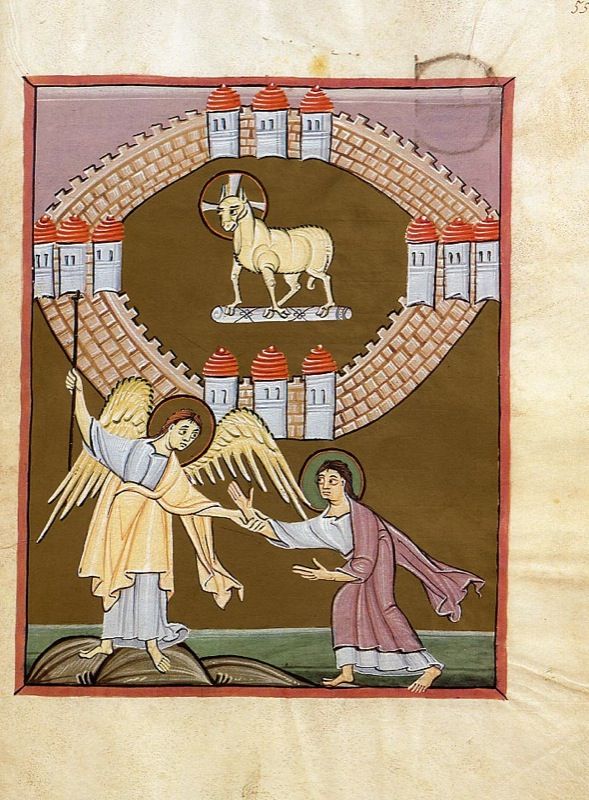
\includegraphics[width=0.54\textwidth]{pictures/tafel39}
\caption{Johannes Apokalypse, Tafel 39, Bramberger Buchmalerei}
\end{center}
\end{figure}

Gesucht wurde eine Methode, die einem Bild den Anschein der Dreidimensionalit\"at verleiht, also ein realistisches Abbild schafft. Die L\"osung fand man in der Entdeckung der Zentralperspektive bzw. perspektivischen Darstellung. Dadurch erhielten die Bilder eine grosse r\"aumliche Tiefe und nat\"urliche Echtheit.

Die mittelalterlichen Malereien waren \glqq konzeptional\grqq, der wichtigste Gegenstand wurde bevorzugt behandelt, selbst wenn dadurch das Bild verzerrt wurde. Typisch f\"ur diesen nicht perspektivischen Malstil ist die Illumination aus dem 12. Jahrhundert eines unbekannten Malers. Die Burg verschwindet fast vor den Schiffen angreifender Krieger, die Schiffe oben im Bild, die sich in weiter Entfernung am Horizont befinden, sind genau so gross wie die Schiffe im Vordergrund.

Die K\"unstler der Renaissance waren meist zugleich Maler, Goldschmiede, Architekten, Ingenieure und Festungsbaumeister. Sie entwarfen und bauten Kirchen, Hospit\"aler, Pal\"aste, Kl\"oster, Br\"ucken, D\"amme, Kan\"ale, Waffen etc. Da sie perspektivische Darstellungen dringend f\"ur die Aus\"ubung ihres Berufes brauchten, fanden diese Artefici notgedrungen L\"osungen f\"ur die Grundprobleme der darstellenden Geometrie. So wurden die K\"unstler des 15. Jahrhunderts auch zu bedeutenden Mathematikern ihrer Zeit.

\textsc{Giottodi Bondone} (1266-1337), \textsc{Van Eyck} (1390-1441), \textsc{Brunelleschi} (1377-1446), \textsc{Alberti} (1404-1472) hatten bereits erste, f\"ur die Zukunft tragbare Erfolge bei der Meisterung des Problems der Perspektive erzielt.

Der Florentiner \textsc{Filippo Brunelleschi}, der ber\"uhmte Baumeister der Domkuppel, beispielsweise wollte \"offentlich beweisen, dass Fl\"achenkunst die Vollkommenheit angewandter Mathematik erreichen kann. Um dies zu beweisen, hatte er unter anderem eine Tafel gemalt, f\"ur die man einen Standort nahe dem Hauptportal und in der Mittelachse des Domes zu w\"ahlen hatte.

Alles, was man von dieser Stelle aus, durch das ge\"offnete Portal hindurch vom Baptisterium und dessen Nachbarbauten sehen konnte, hatte er auf der Tafel mit Farben festgehalten. Die Tafel war in der Mitte vorsichtig gelocht und wurde dem Interessenten zusammen mit einem Spiegel ausgeh\"andigt.

Mit der einen Hand fasste man den Spiegel, mit der anderen die Tafel. Wenn man deren unbemalte R\"uckseite so vors Auge hielt, dass man durch das kleine Loch blicken konnte, und sich gleichzeitig mittels des vor die Vorderseite gehaltenen Spiegels das Gemalte widerspiegeln liess, erhielt man den Eindruck, genau diejenige Wirklichkeit vor
sich zu sehen, die man, wenn der
Spiegel weggenommen wurde, real vor sich sah. Der T\"auschungseffekt war um so erstaunlicher, als er sich sogar auf Bewegliches bezog. Brunelleschi hatte n\"amlich den Himmelsbezirk auf seiner Tafel mit Silberfolie belegt, so dass im Spiegelbild mit der Starrheit der Architektur der Wandel der Wolken kontrastierte. Das Abbild erschien, \"uber alle lineare und farbige †bereinstimmung hinaus, auch noch lebendig.

Die Ideen Brunelleschis wurden von \textsc{Alberti} weiterentwickelt; er schreibt den ersten allgemeinen Traktat \"uber die Perspektive. Zur vollen Meisterschaft in der Kunst der Perspektive brachten es aber erst sp\"ater \textsc{Leonardo da Vinci} (1452- 1519) in Italien und \textsc{Albrecht D\"urer} (1471-1528) in Deutschland.

Der Schl\"ussel zur dreidimensionalen Darstellung liegt in dem Prinzip 'Projektion und Schnitt': Der Maler stellt sich vor, dass von jedem Punkt der zu malenden Szene aus ein Lichtstrahl in sein Auge f\"allt (Zentralprojektion). Zwischen die zu malende Szene und seinem Auge wird
eine Glasscheibe, die seiner Leinwand entspricht, aufgestellt. Auf dieser Glasscheibe werden nun Punkt f\"ur Punkt die Stellen markiert, in denen die Projektions- oder Sehstrahlen die Scheibe durchdringen (Durchstosspunkte). Die Menge aller derartigen Punkte ist ein \glqq Schnitt\grqq. Die Renaissance-K\"unstler hatten entdeckt, dass bei der Betrachtung eines \glqq Schnittes\grqq\ derselbe Eindruck entsteht, als wenn man die Szene direkt anschaut. Denn das Licht, das von einem Objektpunkt ausgeht und in unser Auge f\"allt, verl\"auft geradlinig; die Lichtstrahlen, die von den entsprechenden Punkten auf der Glasscheibe ausgehen, verlaufen auf denselben Geraden. Deshalb muss derselbe Eindruck entstehen. Der Maler hatte jetzt nur noch den \glqq Schnitt\grqq, der auf der Glasscheibe erscheint, auf die Leinwand, die nicht durchsichtig und zweidimensional ist, zu \"ubertragen, um ein realistisches Bild zu erzielen. \textsc{D\"urer} benutzte f\"ur dieses Prinzip das Wort \emph{Perspektive} (perspicere, lat.: hindurchsehen) und illustrierte dies sehr sch\"on auf mehreren Holzschnitten, die aus seinem Lehrbuch \glqq Underweysung der messung mit dem zirkel und richtscheyed \dots\grqq\ (1525) stammen.

\begin{figure}[h!]
\begin{center}
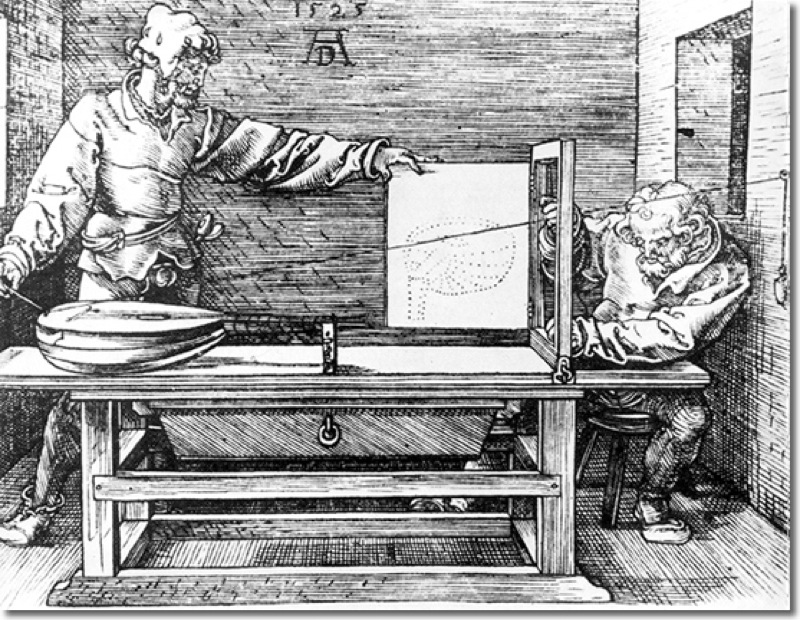
\includegraphics[width=0.618\textwidth]{pictures/durer}
\caption{Aus Albert D\"urers: Underweysung der messun mit dem zirkel und richtscheyed... (1525)}
\end{center}
\end{figure}

Da die Abbildung vom Standpunkt des K\"unstlers und der Placierung der Glasscheibe abh\"angt, gibt es verschiedene Darstellungen von der gleichen Szene. Die dargestellten Objekte k\"onnen verschiedene Gr\"osse haben; ein Bild kann die Szene aus frontaler Sicht zeigen, ein anderes Bild kann dieselbe Szene mehr von der Seite her zeigen. Der Photoapparat ist \"ubrigens ein hervorragendes Beispiel, um das Prinzip "Projektion und Schnitt" zu demonstrieren: Unser Auge, das Projektionszentrum, entspricht der Linse, der 'Schnitt' erscheint auf dem Film. Aus verschiedenen Stellungen erh\"alt man leicht vom gleichen Objekt verschiedene Bilder.

Nach der Wahl des Standpunktes und der Position der Glasscheibe gilt es nun, das Bild auf die Leinwand zu \"ubertragen. Da aber meist die zu malende Szene nur in des K\"unstlers Vorstellung existiert und die Leinwand nicht durchsichtig ist, braucht der K\"unstler Regeln, die stehen durch die Winkel, die die Linien mit der Bildebene bilden. Auf dem Bild von \textsc{Raffael} findet man unter anderem \textsc{Aristoteles, Plato} (mit den Z\"ugen Leonardos), \textsc{Euklid, Epikur, Pythagoras, Empedokles, Heraklit, Diogenes}.

Die erw\"ahnten Grunds\"atze beschreiben nur die einfachsten Dinge, die man wissen muss, um realistisch zu malen. Wie aber erscheinen Kurven auf der Glasscheibe (Leinwand)?
Zum Beispiel zeigt das Bild von \textsc{Lorenzo di Pietro}, dass ein Kreis im allgemeinen nicht als Kreis gemalt werden kann. Er erscheint als Ellipse oder als Parabel- oder Hyperbelbogen auf dem Bild. Dies h\"angt eben davon ab, wo der Kreis sich relativ zum Beobachter befindet. (Stichwort: Kegelschnitte)
Man erkennt, dass realistisches Malen angewandte Mathematik ist. Beim Betrachten eines so konzipierten Bildes sollte man deshalb unbedingt die Position einnehmen, die der Maler bei der Planung des Bildes verwendet hat. Die Bilder der Renaissance-K\"unstler sind meist in Kunstmuseen zu finden, sie k\"onnten genau so gut in naturwissenschaftlichen Museen h\"angen. Liebhaber der Kunst der Renaissance sind bewusst oder unbewusst auch Liebhaber der Naturwissenschaften und der Mathematik!

\begin{figure}[h!]
\begin{center}
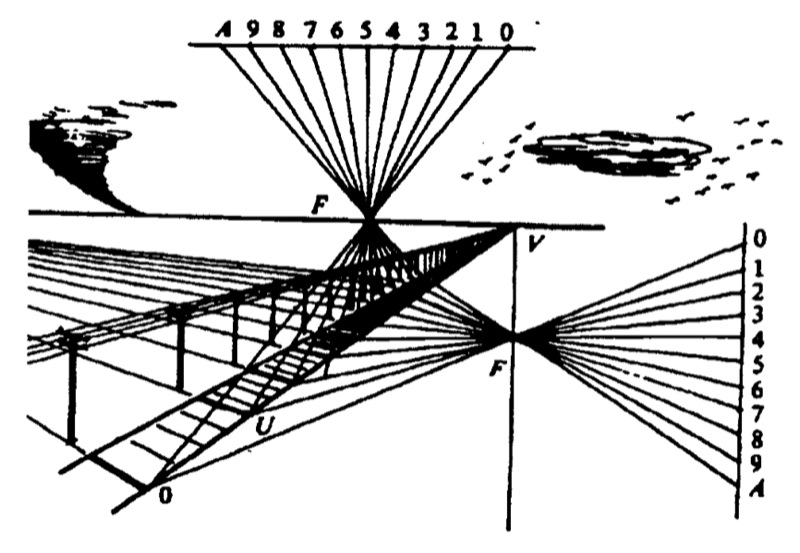
\includegraphics[width=0.618\textwidth]{pictures/eisenbahn}
\end{center}
\caption{Eisenbahn}\label{eisenbahn}
\end{figure}

Abbildung \ref{eisenbahn} zeigt ein konkretes Beispiel, n\"amlich, wie man Eisenbahnschienen mit Schwellen zeichnet, die in eine Landschaft eingebettet sind. Wie sind die Schienen oder die Telegraphenmasten zu positionieren, wo sollen sie im Horizont verschwinden? Man w\"ahlt einen Brennpunkt $F$ verschieden vom Hauptpunkt $V$ und zeichnet die Gerade $FV$. Die Figur zeigt zwei m\"ogliche Wahlen; in dem einen Fall f\"allt $FV$ mit dem Horizont zusammen, im anderen Fall ist $FV$ senkrecht zum Horizont.

Nun nimmt man einen Anfangspunkt $0$ und einen Punkt $U$ auf den Schienen so, dass $OU$ eine Einheitsstrecke wird, an der alle anderen Strecken entlang der Schienen gemessen werden. Als n\"achstes zeichnet man eine Parallele $g$ zu $FV$ und projiziert die Punkte $0$ und $U$ durch $F$ auf $g$. Die Gerade $g$ dient jetzt als perspektivischer Massstab, um die Schwellenabst\"ande entlang der Schienen abzumessen. Eine Folge von \"aquidistanten Punkten auf $g$, zur\"uckprojiziert durch den Brennpunkt $F$ ergibt eine korrekte Perspektive f\"ur die Punkte mit gleichen Abst\"anden auf den Eisenbahnschienen.
Betrachtet man die in der Realit\"at vorhandenen Rechtecke, die aus den beiden Schienen und je zwei Schwellen gebildet werden, so erkennt man:

Das Bild ist weder kongruent, noch \"ahnlich, noch fl\"achengleich zu der Originalfigur.
Die Perspektive ist nicht winkeltreu.

Die Bilder seit der Renaissance zeigen, dass man die geometrische Struktur des Originals auf der Leinwand gut erkennen kann. Dies liegt darin begr\"undet, dass es geometrische Eigenschaften gibt, die invariant gegen\"uber Projektionen sind, also Eigenschaften, die im Bild unver\"andert erscheinen und daher ihre Identifizierung erm\"oglichen. Diese Eigenschaften aufzuzeigen und zu untersuchen ist die Aufgabe der projektiven Geometrie. Eine der fr\"uhesten Entdeckungen der projektiven Geometrie ist der ber\"uhmte Dreieckssatz des franz\"osischen Architekten und Ingenieurs \textsc{Gerard Desargues} (1593-1662). Dieser Satz zeigt die signifikante Eigenschaft, die zwei Schnitten derselben Projektion eines Dreiecks zukommt.

Wenn zwei Dreiecke $ABC$ und $A'B'C'$ in zwei verschiedenen, aber nicht parallelen Ebenen so gelegen sind, dass die Verbindungslinien einander entsprechender Punkte in einem Punkt $0$ kongruent sind (die Dreiecke befinden sich in perspektiver Lage), dann schneiden sich die Verl\"angerungen entsprechender Seiten in drei kollinearen Punkten $R$, $S$ und $T$.

Der Satz von \textsc{Desargues} ist auch richtig, wenn die beiden Dreiecke in einer Ebene liegen.

Die Bilder seit der Renaissance zeigen, dass man die geometrische Struktur des Originals auf der Leinwand gut erkennen kann. Dies liegt darin begr\"undet, dass es geometrische Eigenschaften gibt, die invariant gegen\"uber Projektionen sind. Diese Eigenschaften aufzuzeigen und zu untersuchen ist Aufgabe der projektiven Geometrie.

\begin{ueb}
Wie lautet der Dreieckssatz von \textsc{Gerard Desargues}? Skizzieren Sie die Situation.
\end{ueb}

\begin{figure}[h!]
\begin{center}
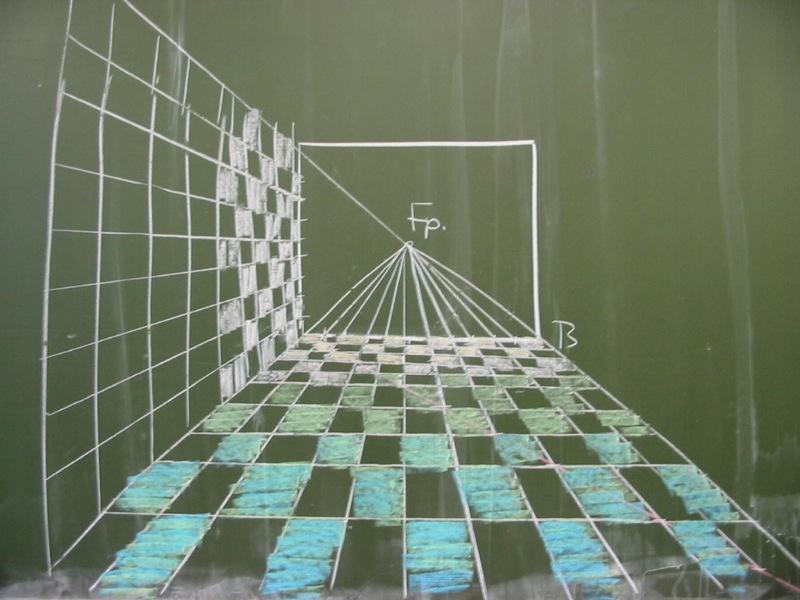
\includegraphics[width=0.8\textwidth]{pictures/fluchtp}
\caption{Wandtafelskizze zur Konstruktion des Fluchtpunktes}
\end{center}
\end{figure}

Viele K\"unstler machen sich die Theorien der Perspektive zu nutze oder spielen damit. Hier noch einige Beispiele:

\begin{figure}[h!]
\begin{center}
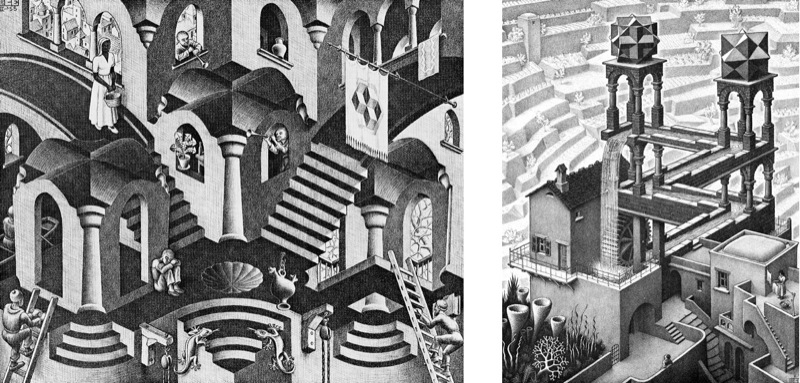
\includegraphics[width=0.618\textwidth]{pictures/escher}
\caption{Bilder von \textsc{Escher}}
\end{center}
\end{figure}

\begin{figure}[h!]
\begin{center}
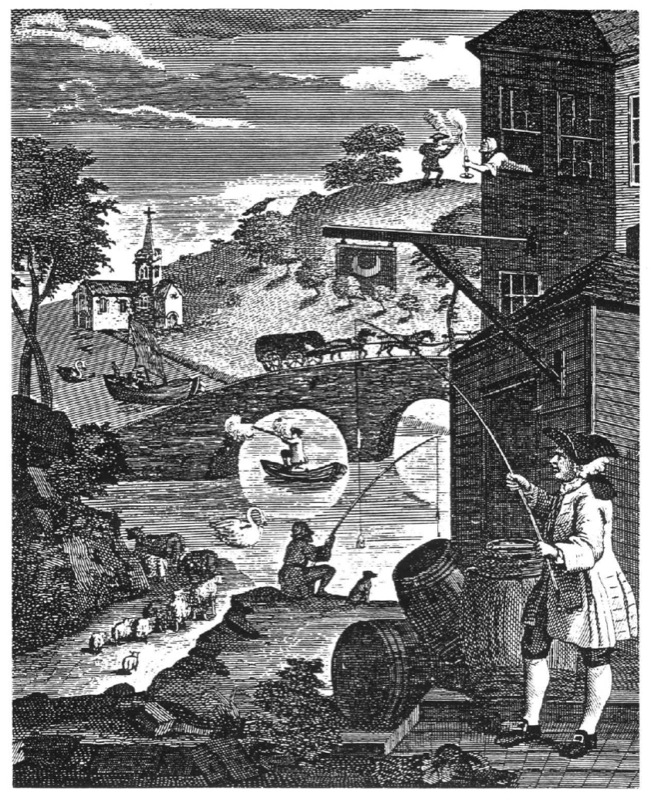
\includegraphics[width=0.618\textwidth]{pictures/hogarth}
\caption{Bild von \textsc{William Hogarth} (1697--1764)}
\end{center}
\end{figure}

\vfill

\section*{L\"osungen}

1.) Die Verbindungslinien zwischen korrespondierenden Eckpunkten zweier in einer Ebene liegenden Dreiecke schneiden sich in einem Punkt genau dann, wenn die Schnittpunkte der entsprechenden verl\"angerten Seiten auf einer Geraden liegen.

\clearpage

\section{Stereometrie}
\begin{wrapfigure}{r}{0.382\textwidth}
  \begin{center}
    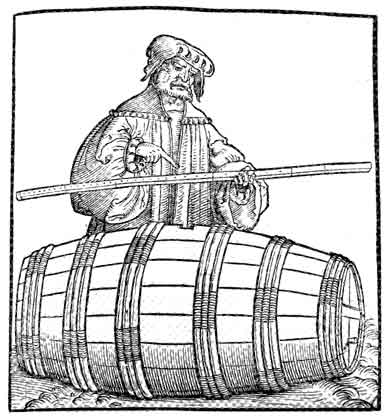
\includegraphics[width=0.382\textwidth]{pictures/fass}
  \end{center}
%\caption{A gull}
\end{wrapfigure}
Die Stereometrie (griech., K\"orpermessung) besch\"aftigt
sich im Gegensatz zur Planimetrie mit der Form, gegenseitigen Lage und Gr\"osse geometrischer Gebilde des Raumes. Im engeren Sinne ist sie die Lehre von der Ausmessung der K\"orper.

K\"orper sind Teile des Raumes, die durch ihre Oberfl\"ache vom \"ubrigen Raum abgegrenzt werden. K\"orper haben also ein bestimmtes Volumen und eine bestimmte Oberfl\"ache.
Die einfachen K\"orper --- W\"urfel, Quader, Zylinder, Kugel --- waren schon bei allen V\"olkern der vorgeschichtlichen Zeit bekannt und wurden praktisch genutzt (Hausbau, Fruchtspeicher, Gef\"asse, religi\"ose Zwecke etc.). Sowohl die Babyionier (3500 bis 200 v.u.Z.) als auch die \"Agypter (3000 bis 500 v.u.Z.) haben Volumen und Oberfl\"ache von W\"urfeln, Zylindern, Pyramiden, Pyramidenst\"umpfen, Kegeln und prismatischen K\"orpern, wenn auch teilweise nur in guter N\"aherung, berechnen k\"onnen. \textsc{Euklid} (350 v.u.Z.) f\"uhrte die ersten planm\"assigen, rein mathematischen Untersuchungen durch. Die Berechnung des Volumens und der Oberfl\"ache einer Kugel gelang aber erst Archimedes (287 - 212 v.u.Z.).

\subsection{Volumen und Oberfl\"ache}
\subsubsection{Prismen}
\begin{ueb}
Berechne Volumen $V$, Oberfl\"ache $O$ und Raumdiagonale $d$ eines
\begin{enumeratea}
\item W\"urfels mit Kantenl\"ange $k$
\item eines Quaders mit Kantenl\"ange $a,b,c$
\end{enumeratea}
\end{ueb}

\subsubsection{Pyramiden}
\begin{ueb}
Die Cheopspyramide hat als Grundfl\"ache ein Quadrat mit Seitenl\"ange $\unit[233]{m}$. Sie war urspr\"unglich $\unit[148]{m}$ hoch; heute ist sie auf einer H\"ohe von $\unit[137]{m}$ abgestumpft.
\begin{enumeratea}
\item Der Bau soll $\unit[100000]{Mann}$ $\unit[20]{Jahre}$ besch\"aftigt haben. Welche Gesteinsmasse wurde dabei bewegt? (Dichte des Gesteins: $\rho_S=\unitfrac[2.7]{g}{cm^3}$)
\item Welche Abmessung hat die heutige Plattform?
\end{enumeratea}

\begin{figure}[h!]
\begin{center}
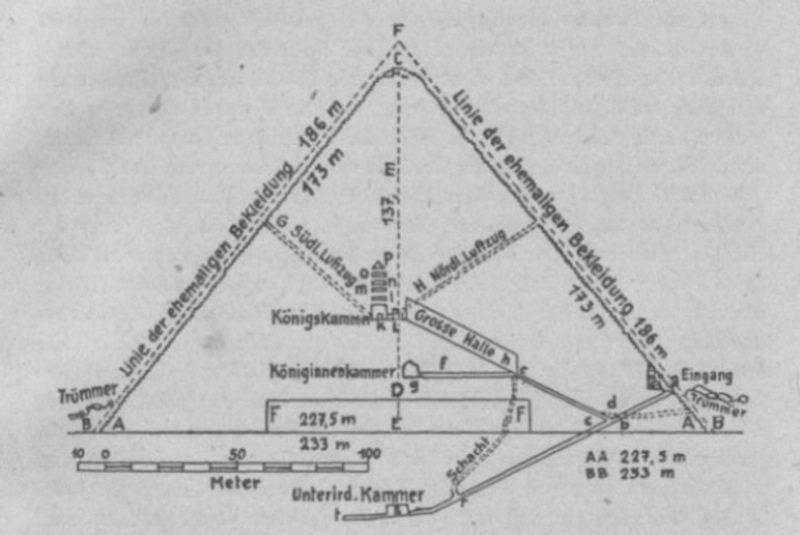
\includegraphics[width=0.9\textwidth]{pictures/cheops}
\caption{Cheopspyramide}
\end{center}
\end{figure}

\end{ueb}

\begin{ueb}
Ein Zelt hat die Gestalt eines regelm\"assigen sechsseitigen Pyramidenstumpfs mit den Grundkanten $a=\unit[4.8]{m}$ und $b=\unit[3.6]{m}$. Die Seitenkante misst jeweils $s=\unit[2.4]{m}$.
\begin{enumeratea}
\item Welchen Raum umschliesst das Zelt?
\item Wieviel Zeltstoff war zur Herstellung n\"otig?
\end{enumeratea}
\end{ueb}

\subsubsection{Gerader Kreiszylinder}
\begin{ueb}
Ein rechteckiges Blatt mit den Seitenl\"angen $a$ und $b$ kann auf zwei Arten zu einem Zylinder gebogen werden. Wie gross ist das Verh\"altnis der \\[1ex]
\hspace*{2.7ex}(a) Volumina$\q$ (b) M\"antel
\end{ueb}

\begin{ueb}
Eine Plakats\"aule ist $\unit[2.6]{m}$ hoch und hat einen Durchmesser von $\unit[1.2]{m}$. Wie gross ist die m\"ogliche Reklamefl\"ache?
\end{ueb}

\begin{ueb}
Wie viel Blech ben\"otigt man f\"ur eine Konservendose (Durchmesser $\unit[10]{cm}$, Inhalt $\unit[1]{Liter}$), wenn f\"ur Verschnitt etc. noch 15\% zugeschlagen werden?
\end{ueb}

\begin{ueb}
Eine Rolle Eisendraht (Dichte: $\unitfrac[7.8]{g}{cm^3}$) wiegt $\unit[135]{N}$. Wie lang ist der Draht, wenn seine Dicke $\unit[2.4]{mm}$ betr\"agt?
\end{ueb}

\begin{ueb}
Die Metallverkleidung eines Kamins muss mit einer Spezialfarbe zweimal gestrichen werden. Die Kaminverkleidung ist ein Zylinder mit einem Durchmesser von $\unit[150]{cm}$ und einer H\"ohe von $\unit[18]{m}$. Beim ersten Anstrich rechnet man mit $\unit[1]{kg}$ Farbe f\"ur $\unit[15]{m^2}$; beim zweiten Anstrich gen\"ugen 70\% der Menge des ersten Anstrichs. Wie viele Dosen (ˆ $\unit[5]{kg}$ bzw. $\unit[10]{kg}$) Farbe werden ben\"otigt?
\end{ueb}

\begin{ueb}
Zeichne die Parabel mit der Gleichung $y=4-x^2$ f\"ur $-2<x<2$. Lasse das Parabelst\"uck um die y-Achse rotieren, so dass ein Paraboloid entsteht, und berechne dessen Volumen. Hinweis: Betrachte einen Zylinder mit dem Radius 2 und der H\"ohe 4, aus dem ein kongruentes Rotationsparaboloid --- durch die Parabel $y=x^2$ entstanden --- herausgefr\"ast wird, und wende das Prinzip von Cavalieri an.
\end{ueb}

\subsubsection{Gerader Kreiskegel}
\begin{ueb}
Von einem geraden Kreiskegel kennt man den Radius $r=\unit[5]{cm}$ und das Volumen $V=\unit[1000]{cm^3}$. Berechne $h$, $s$, $M$ und $O$.
\end{ueb}

\begin{ueb}
Wie tief taucht ein Holzkegel ($r=\unit[5]{cm}$, $h=\unit[12]{cm}$, Dichte $\unitfrac[0.8]{g}{cm^3}$) mit der Spitze nach unten in Wasser ein?
\end{ueb}

\begin{ueb}
Wie gross ist der Mittelpunktswinkel des Kreisausschnittes, der den abgewickelten Mantel eines Kegels mit r=6 cm und h=8 cm darstellt?
\end{ueb}

\begin{ueb}
Ein Kreisausschnitt mit dem Mittelpunktswinkel 120¡ und dem Radius $\unit[8]{cm}$ wird zu einem Kegel zusammengebogen. Wie gross wird dessen Volumen?
\end{ueb}

\subsubsection{Kugel}
Die Berechnung des Volumens der Kugel erfolgt mit dem Prinzip von Cavalieri. Als Vergleichsk\"orper nimmt man denjenigen K\"orper, der entsteht, wenn man aus einem Zylinder (Radius $r$, H\"ohe $r$) einen Kegel herausfr\"ast.
Man schneidet die Halbkugel und den Vergleichsk\"orper mit einer Ebene, die vom Mittelpunkt der Kugel den Abstand $a$ hat. Als Schnittfl\"achen ergeben sich
f\"ur die Halbkugel
$$A = \pi r'^2 =\pi(r^2 - a^2),$$
f\"ur den Vergleichsk\"orper
$$A =A_{Kreisring} =\pi r^2-\pi a^2$$
F\"ur das Volumen der Kugel gilt deshalb:
\begin{align*}
V_{Halbkugel}&=V_{Zylinder}-V_{Kegel}\\
&=\pi r^3-\frac{1}{3}\pi r^3=\frac{2}{3}\pi r^3,
\end{align*}
also
$$V_{Kugel}=\frac{4}{3}\pi r^3.$$

\begin{ueb}
Berechne den Radius einer Kugel mit $\unit[1]{m^3}$ Rauminhalt.
\end{ueb}

\begin{ueb}
Leite eine Formel f\"ur das Materialvolumen einer Hohlkugel in Abh\"angigkeit vom Kugelradius rund der Wanddicke $d$ her. Welche Glieder der Formel k\"onnen bei sehr kleinem $d$ vernachl\"assigt werden? Deute die entstehende N\"aherungsformel und leite somit die Formel f\"ur die Oberfl\"ache einer Kugel ab.
\end{ueb}

\begin{ueb}
Der Inhalt der Gesamtaustauschfl\"ache der menschlichen Lunge betr\"agt ungef\"ahr $\unit[140]{m^2}$. Wie viele kugelf\"ormige (durchschnittlicher Durchmesser $\unit[0.3]{mm}$) Lungenbl\"aschen besitzt demnach ein Mensch?
\end{ueb}

\begin{ueb}
Wie verhalten sich die\\[1ex]
\hspace*{2.7ex}(a) Radien$\q$ (b) Oberfl\"achen$\q$ (c) Volumina\\[1ex]
der In- und Umkugel eines W\"urfels?
\end{ueb}

\begin{ueb}
Die Figur hat Archimedes in seinen Grabstein meisseln lassen.
\begin{center}
\definecolor{zzttqq}{rgb}{0.6,0.2,0}
\scalebox{0.85}{
\begin{tikzpicture}[line cap=round,line join=round,>=triangle 45,x=0.7cm,y=0.7cm]
\clip(-4.62,-2.54) rectangle (4.96,6.54);
\draw(0,2) circle (2.8cm);
\draw [color=zzttqq] (-4,6)-- (4,6);
\draw [color=zzttqq] (4,6)-- (4,-2);
\draw [color=zzttqq] (4,-2)-- (-4,-2);
\draw [color=zzttqq] (-4,-2)-- (-4,6);
\draw [color=zzttqq] (0,6)-- (-4,-2);
\draw [color=zzttqq] (-4,-2)-- (4,-2);
\draw [color=zzttqq] (4,-2)-- (0,6);
\end{tikzpicture}
}
\end{center}
Der R\"omer Cicero hat eineinhalb Jahrhunderte nach dem Tode von Archimedes dessen Grab an diesem Zeichen erkannt. Worauf soll dieses Zeichen wohl aufmerksam machen?
\end{ueb}

\begin{ueb}
Ein kugelf\"ormiger …ltropfen von $\unit[4]{mm}$ Durchmesser breitet sich auf einer Wasseroberfl\"ache zu einer Schicht von $\unit[1.2]{m^2}$ Fl\"acheninhalt aus. Berechne die H\"ohe dieser Schicht.
\end{ueb}

\section*{L\"osungen}

1.) $k^3$, $6k^2$, $\sqrt{3}k$; $abc$, $2(ab+ac+bc)$, $\sqrt{a^2+b^2+c^2}$.

2.) \"uber $\unit[7]{Mio. Tonnen}$; knapp $\unit[300]{m^2}$.

3.) $\unit[96]{m^3}$; $\unit[71.5]{m^2}$

4.) $a\div b$; $1\div1$.

5.) $\unit[9.8]{m^2}$

6.) $\unit[6.4]{dm^2}$

7.) $\unit[390]{m}$

8.) $10$ K\"ubel

9.) $16.76$

10.) $h=\frac{3V}{\pi r^2}$, $s=\sqrt{h^2+r^2}$, $M=\pi rs$, $O=M+\pi r^2$

11.) $\unit[11.14]{cm}$

12.) $216^\circ$

13.) $\unit[1516.5]{cm^3}$

14.) $\unit[0.62]{m^3}$

15.) $\frac{4}{3}\pi(3r^2d-3rd^2+d^3)$

16.) $\unit[124]{Mio.}$

17.) $1\div\sqrt{3}$; $1\div 3$; $1\div 3\sqrt{3}$.

18.) Kegel$\div$Kugel$\div$Zylinder$=1\div2\div3$.

19.) $\unit[28]{nm}$

\section{Polyeder}
Als Polyeder (griech., Vielfl\"achner) bezeichnet man K\"orper, die nur von ebenen Vielecken begrenzt werden. Beispiele sind W\"urfel, Pyramiden, Prismen; ein Zylinder ist kein Polyeder.

Besteht eine Oberfl\"ache eines konvexen Polyeders aus lauter kongruenten Vielecken und treffen in dessen Ecken immer die gleiche Anzahl Fl\"achen zusammen, so spricht man von \emph{regelm\"assigen Polyedern}. Ihre Anzahl ist beschr\"ankt und kann ermittelt werden, wenn man bedenkt:
\begin{itemize}
\item Die Summe aller Kantenwinkel an jeder K\"orperecke muss kleiner als $360¡$ sein.
\item In jeder K\"orperecke stossen mindestens $3$ Fl\"achen zusammen.
\end{itemize}
Somit folgt: Wird das Polyeder von regelm\"assigen Dreiecken begrenzt, so kann eine Ecke nur von $3$, $4$ oder $5$ Seitenfl\"achen gebildet werden (Tetraeder, Oktaeder, Ikosaeder). Wird das Polyeder von regelm\"assigen Vierecken (Hexaeder) oder regelm\"assigen F\"unfecken (Dodekaeder) begrenzt, so kann eine Ecke nur durch $3$ Seitenfl\"achen gebildet werden. Andere M\"oglichkeiten gibt es nicht mehr.
\begin{ueb}
Begr\"unden Sie diese Folgerungen.
\end{ueb}
\begin{satz}
Es gibt genau $5$ regelm\"assige Polyeder.
\end{satz}

\begin{figure}[h!]
\begin{center}
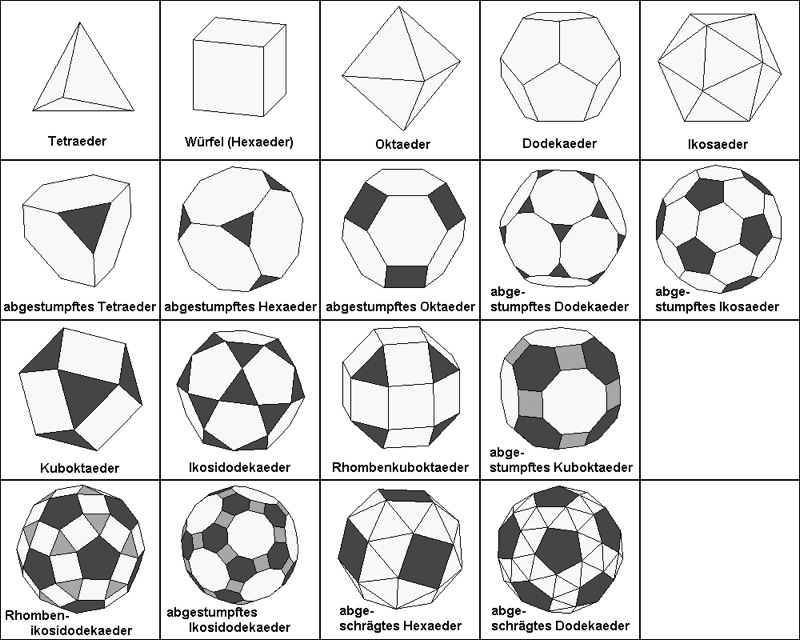
\includegraphics[width=0.8\textwidth]{pictures/polyeders}
\end{center}
\caption{Die f\"unf regelm\"assigen Polyeder mit verwandten}
\end{figure}

F\"ur den griechischen Philosophen \textsc{Plato} (427--347 v.~Chr.) waren diese f\"unf K\"orper Grundbausteine seines Weltsystems: Sie entsprachen den vier Elementen Feuer, Erde, Wasser und Luft. Das Dodekaeder entsprach einer Schale, die das ganze Universum einh\"ullt. Daher werden die f\"unf regelm\"assigen Polyeder auch \emph{platonische K\"orper} genannt.

\begin{figure}[h!]
\begin{center}
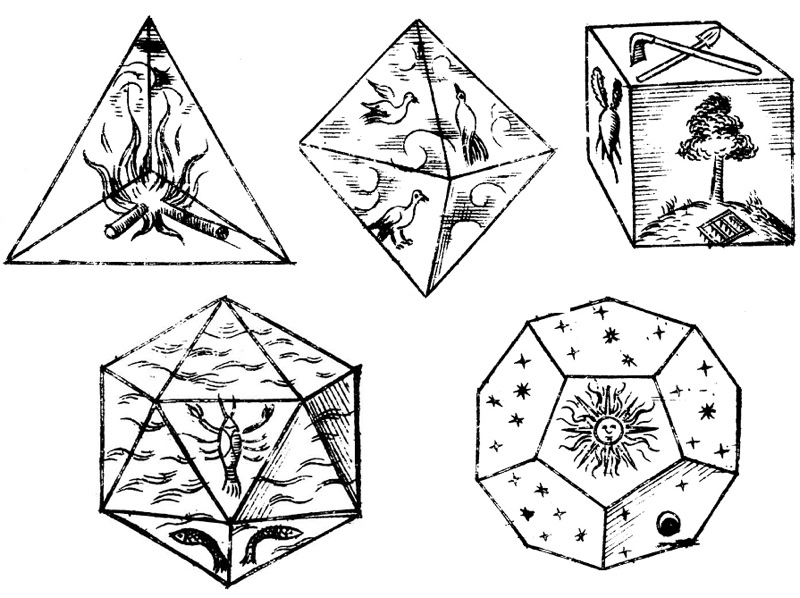
\includegraphics[width=0.95\textwidth]{pictures/platonkoerper}
\end{center}
\caption{Die f\"unf platonischen K\"orper und ihre Bedeutung als Elemente}
\end{figure}

Diese Idee Platons kann als erster bekannter Versuch interpretiert werden, die Welt mit einem Atombild zu erkl\"aren. \textsc{Platon} stellte auch Regeln auf, wie die einzelnen Elemente miteinander reagieren oder ineinander \"ubergef\"uhrt werden k\"onnen.

Die platonischen K\"orper beeindrucken durch ihre vollkommene Gestalt; selbst die Natur bevorzugt beispielsweise bei Kristallformen deren Gestalt.
\begin{figure}
\begin{center}
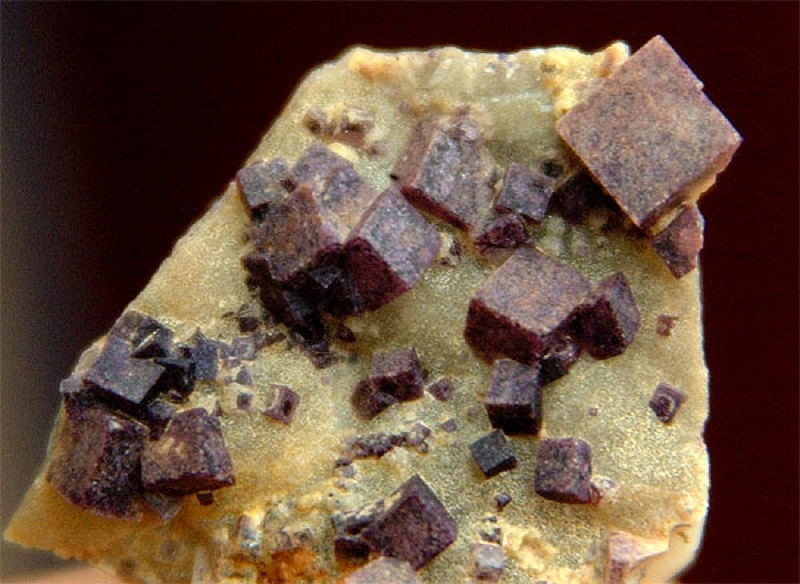
\includegraphics[width=0.7\textwidth]{pictures/kristallh}
\end{center}
\caption{Fluorkristalle (W\"urfel)}
\end{figure}

\begin{figure}
\begin{center}
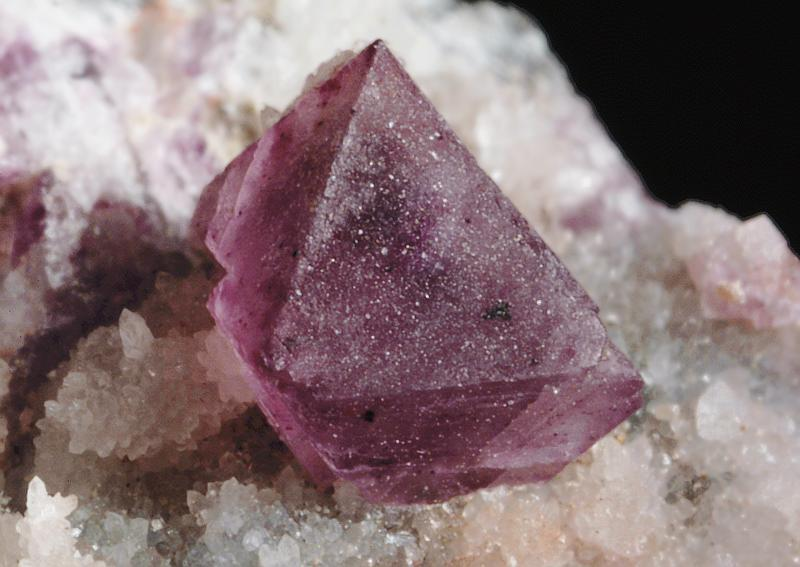
\includegraphics[width=0.7\textwidth]{pictures/kristallo}
\end{center}
\caption{Fluorkristalle (Oktaeder) auf Quarzkristallrasen}
\end{figure}
Der Astronom \textsc{Johannes Kepler} (1471--1528) benutzte diese regelm\"assigen Polyeder als Modell f\"ur die Bahnen der Planeten.
\begin{figure}
\begin{center}
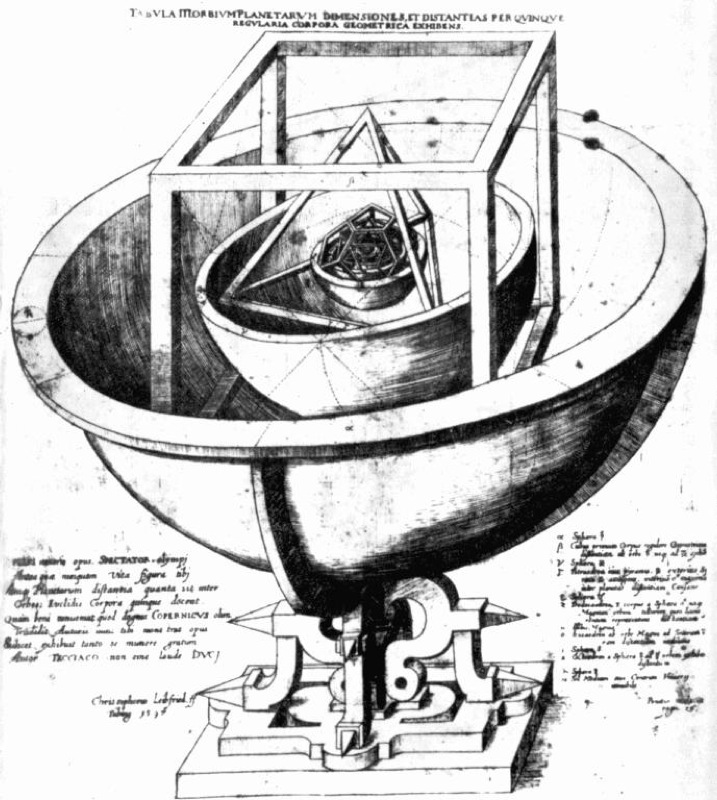
\includegraphics[width=0.9\textwidth]{pictures/kepler}
\end{center}
\caption{Planetenbahnmodell von \textsc{Kepler}}
\end{figure}
Eine der Erdbahn zugeordnete Kugel bildet den Ausgang. Ihr wird ein Dodekaeder umbeschrieben; auf dessen Umkugel liegt die Bahn des Mars. Das dieser Kugel umbeschriebene Tetraeder enth\"alt auf seiner Umkugel die Bahn des Jupiter, und der dieser Kugel umbeschriebene W\"urfel bestimmt eine Umkugel, auf der die Bahn des Saturn verl\"auft. Das der Erdbahnkugel einbeschriebene Ikosaeder tr\"agt auf seiner Inkugel die Bahn der Venus und das dieser Inkugel einbeschrieben Oktaeder enth\"alt auf seiner Inkugel die Bahn des Merkurs.

\begin{ueb}
Welche der Figuren stellen aufgeklappte W\"urfel dar?
\begin{figure}[h!]
\begin{center}
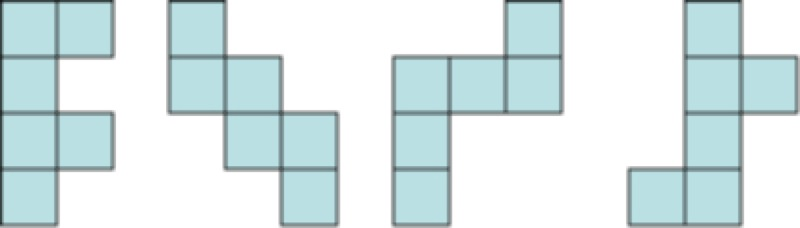
\includegraphics[width=0.9\textwidth]{pictures/wuerfelnetz}
\end{center}
\caption{W\"urfelnetze}
\end{figure}
\end{ueb}

\begin{ueb}
Besorge dir ein mittelstarkes glattes farbiges Zeichenpapier, ein Eisenlineal und ein Messer zum Schneiden und Einritzen. Zeichne die Netze der platonischen K\"orper und bauen Sie sich saubere Modelle.
\end{ueb}

\begin{ueb}
Zeichne zu jedem platonischen K\"orper ein Schr\"agbild. Benutzen Sie beim tetraeder, Oktaeder und Ikosaeder einen W\"urfel, der diesen K\"orper umgibt, beim Dodekaeder einen W\"urfel, der innerhalb des Dodekaeders liegt. Vergleichen Sie mit den Modellen aus der Schulsammlung.
\end{ueb}

\begin{ueb}
F\"ullen Sie folgende Tabelle aus:
\begin{center}
\begin{tabular}{|c|c|c|c|}\hline
\spaltenheight\textbf{K\"orper} & \textbf{Ecken} & \textbf{Fl\"achen} & \textbf{Kanten}\spaltensep \hline
\spaltenheight Tetraeder & & & \spaltensep \hline
\spaltenheight Hexaeder & & & \spaltensep \hline
\spaltenheight Oktaeder & & & \spaltensep \hline
\spaltenheight Dodekaeder & & & \spaltensep \hline
\spaltenheight Ikosaeder & & & \spaltensep \hline
\end{tabular}
\end{center}
Erkl\"are die Namen der platonischen K\"orper. Was f\"allt bei den Zahlen in der Tabelle auf? Bestimme zus\"atzlich alle Symmetrien.
\end{ueb}

\subsection{Der Euler'sche Polyedersatz}
Obwohl sich die griechischen Mathematiker intensiv mit den Polyedern besch\"aftigt haben, wurde der folgende Satz erst von \textsc{Leonard Euler} (1707--1783) entdeckt.
\begin{satz}
Es sei $E$ die Anzahl Ecken, $K$ die Anzahl Kanten und $F$ die Anzahl Seitenfl\"achen eines beliebigen Polyeders. Dann gilt:
$$E-K+F=2.$$
\end{satz}
\begin{proof}[Beweis]
Wir haben diesen Satz bereits bei den platonischen K\"orper best\"atigt. Die folgenden Beweisschritte werden am Beispiel eines W\"urfels demonstriert. Man stelle sich dabei vor, dass die Oberfl\"ache des Polyeders aus einer Gummihaut besteht.

\begin{minipage}{0.618\textwidth}
\begin{enumerate}
\item Nach Herausnehmen einer Fl\"ache ($F\rightarrow F-1$) kann man die Oberfl\"ache so stark deformieren, dass sie schliesslich flach in der Ebene liegt.\\
\item Triangulation: In jedem Vieleck, das nicht schon ein Dreieck ist, wird eine Diagonale eingezeichnet: ($K\rightarrow K+1, F\rightarrow F+1$) $E-K+F$ bleibt konstant.\\
\item Bei den Dreiecken, die nur eine Kante auf der Randlinie haben, wird alles entfernt, was nicht zugleich zu anderen Dreiecken geh\"ort: ($K\rightarrow K-1, F\rightarrow  F-1$) $E-K+F$ bleibt konstant.\\
\item Bei den Dreiecken, die zwei Kanten auf der Randlinie haben, wird auch alles entfernt, was nicht zugleich zu anderen Dreiecken geh\"ort: ($E\rightarrow  E-1, K\rightarrow  K-2, F\rightarrow  F-1$) $E-K+F$ bleibt konstant.\\
\item Die Punkte 3. und 4. werden so lange wiederholt, bis zuletzt nur noch ein Dreieck mit $E-K+F=1$ \"ubrig bleibt.\\
\end{enumerate}
\end{minipage}
\hspace*{2cm}
\begin{minipage}{1.7cm}
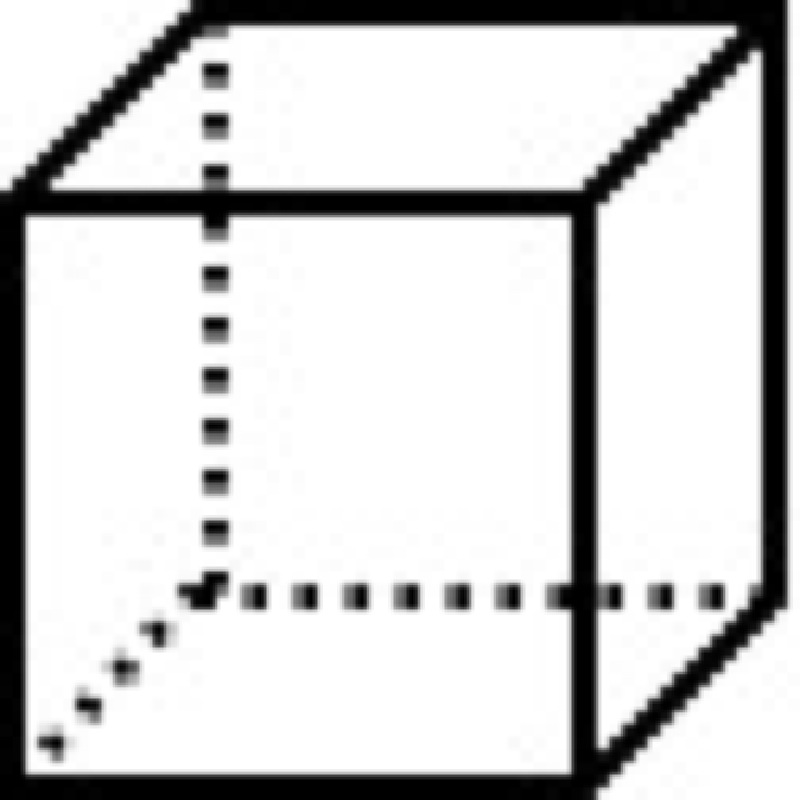
\includegraphics[width=1.7cm]{pictures/wuerf1}\\[3ex]
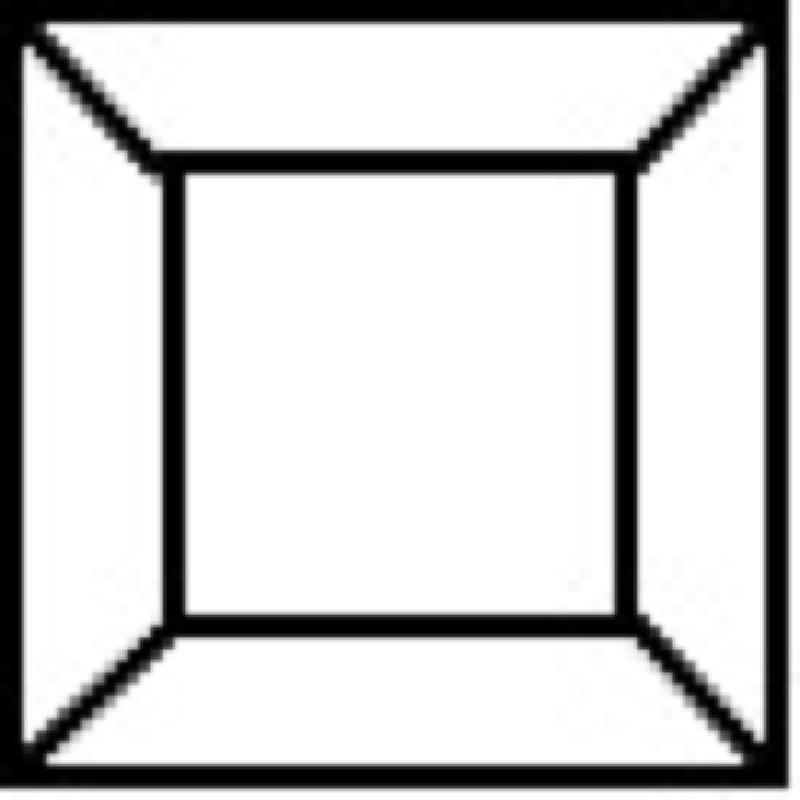
\includegraphics[width=1.7cm]{pictures/wuerf2}\\[4ex]
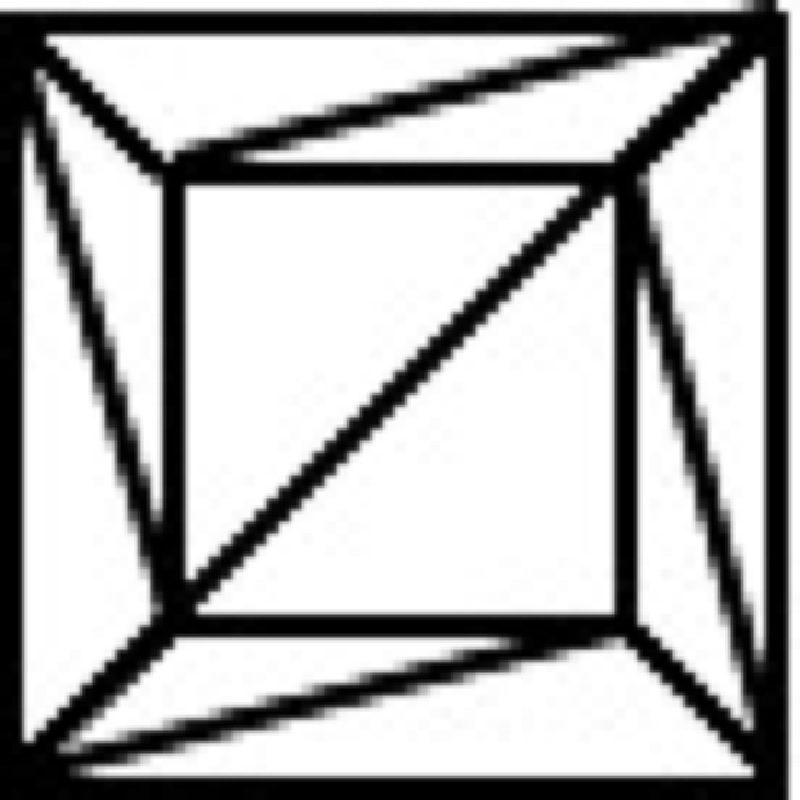
\includegraphics[width=1.7cm]{pictures/wuerf3}\\[5ex]
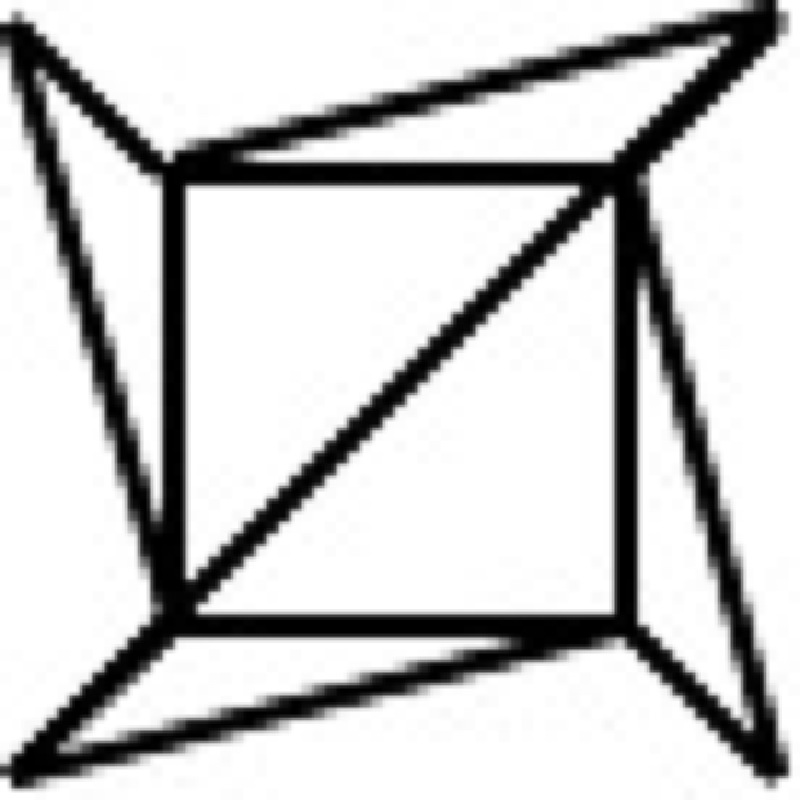
\includegraphics[width=1.7cm]{pictures/wuerf4}\\[6ex]
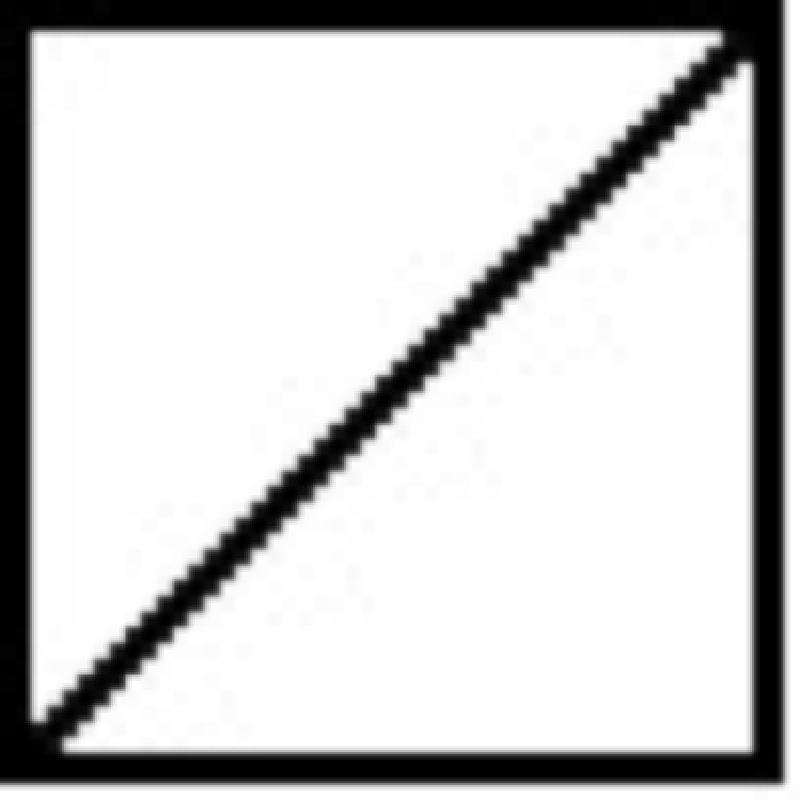
\includegraphics[width=1.7cm]{pictures/wuerf5}\\[7ex]
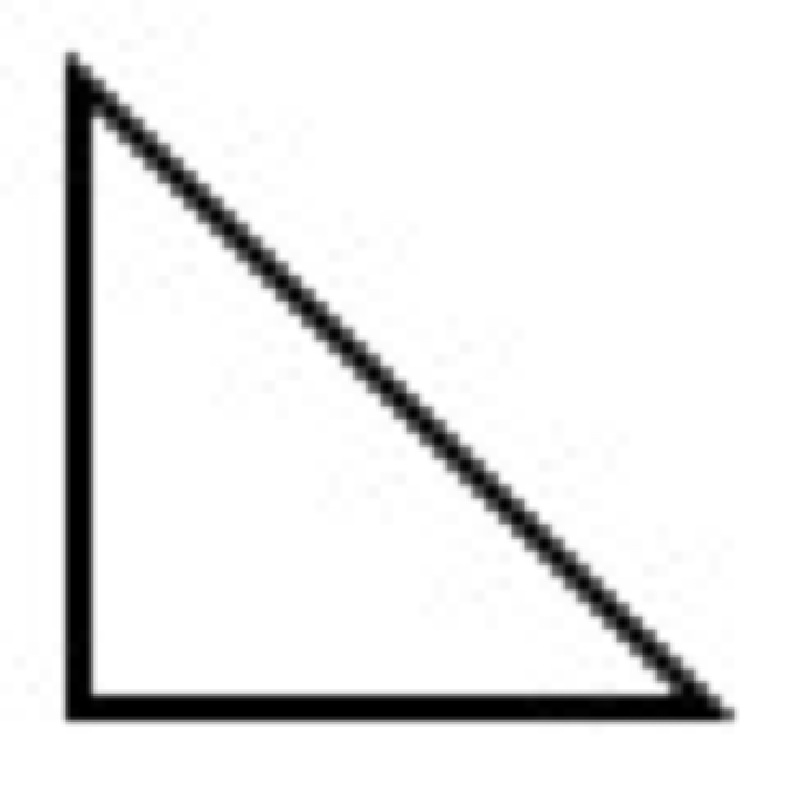
\includegraphics[width=1.7cm]{pictures/wuerf6}
\end{minipage}\\
Bei diesen Operationen hat sich der Wert von $E-K+F=1$ nicht ver\"andert. Ber\"ucksichtigt man noch Punkt 1., so muss f\"ur das Polyeder $E-K+F=2$ gelten.
\end{proof}

\begin{ueb}
Zeichne die entsprechende Beweisfiguren f\"ur das Tetraeder.
\end{ueb}

\begin{ueb}
Ein konvexes Polyeder hat 14 Fl\"achen und 24 Ecken. Wie viele Kanten hat es?
\end{ueb}

\section*{L\"osungen}

1.) klar

2.) f, \checkmark, f, \checkmark

5.) $4,4,6$; $8,6,12$; $6,8,12$; $20,12,30$; $12,20,30$.

7.) $36$

\section{Polarkoordinaten}
Die Lage eines Punktes $P$, verschieden von $\point{0}{0}$, in einem rechtwinkligen Koordinatensystem kann nicht nur durch seine kartesischen Koordinaten $\point{x}{y}$, sondern auch durch seinen Abstand $r>0$ vom Ursprung und einem Richtungswinkel $\varphi\in[0,2\pi)$ eindeutig angegeben werden.
\begin{center}\definecolor{qqwuqq}{rgb}{0,0.39,0}
\scalebox{1.1}{
\begin{tikzpicture}[line cap=round,line join=round,>=triangle 45,x=0.5cm,y=0.5cm]
\draw[->,color=black] (-2.78,0) -- (10,0);
\foreach \x in {-2,-1,1,2,3,4,5,6,7,8,9}
\draw[shift={(\x,0)},color=black] (0pt,2pt) -- (0pt,-2pt);
\draw[color=black] (9.66,0.08) node [anchor=south west] {$x$};
\draw[->,color=black] (0,-2.28) -- (0,8.3);
\foreach \y in {-2,-1,1,2,3,4,5,6,7,8}
\draw[shift={(0,\y)},color=black] (2pt,0pt) -- (-2pt,0pt);
\draw[color=black] (0.1,7.9) node [anchor=west] {$y$};
\clip(-2.78,-2.28) rectangle (10,8.3);
\draw [shift={(0,0)},line width=1.6pt,color=qqwuqq,fill=qqwuqq,fill opacity=0.1] (0,0) -- (0:2) arc (0:44.22:2) -- cycle;
\draw [line width=2pt] (5.92,5.76)-- (0,0);
\fill [color=black] (5.92,5.76) circle (1.5pt);
\draw[color=black] (6.2,6.2) node {$P$};
\draw[color=black] (2.76,3.26) node {$r$};
\draw[color=qqwuqq] (1.26,0.5) node {$\varphi$};
\end{tikzpicture}
}
\end{center}
Das Paar $\point{r}{\varphi}$ nennt man die \textbf{Polarkoordinaten} von $P$.

\begin{ueb}
Stelle Formeln f\"ur die Umrechnung von kartesischen Koordinaten $\point{x}{y}$ in Polarkoordinaten und vice versa auf.
\end{ueb}

\begin{ueb}
Berechne die Polarkoordinaten der Punkte $K_1=\point{3}{0}$ und $K_2=\point{-3}{-4}$, sowie die kartesischen Koordinaten der Punkte $P_1=\point{7}{\frac{\pi}{2}}$ und $P_2=\point{5}{\frac{7\pi}{4}}$.
\end{ueb} 

\begin{ueb}
Zeichne die Kurven der Gleichungen. Benutze gegebenenfalls eine Wertetabelle.

  \begin{minipage}{3.5cm}
    \begin{enumeratea}
      \item $r=4$
      \item $\varphi=60¡$
      \item $r=\cos(2\varphi)$
    \end{enumeratea}
  \end{minipage}
  \begin{minipage}{4cm}
    \begin{enumeratea}\addtocounter{enumi}{3}
      \item $r=10\sin(3\varphi)$
      \item $r=5(1-\cos\varphi)$
      \item $r=4\cos(2\varphi)/\cos\varphi$
    \end{enumeratea}
  \end{minipage}
\end{ueb}

\begin{ueb}
Zeichne die Kurve, die durch folgende Parametergleichung gegeben ist
\begin{align}
x&=2(t-\sin t)\notag\\
y&=2(1-\cos t)\notag
\end{align}
mit $t\in\D{R}$.
Diese Kurve wird als \emph{Helena der Mathematik} bezeichnet.
\end{ueb}

\section*{L\"osungen}

\hspace*{2.7ex} 1.) $\point{\sqrt{x^2+y^2}}{\tan^{-1}(\frac{y}{x})}$; $\point{r\cos\varphi}{r\sin\varphi}$

2.) $\point{3}{0¡}$, $\point{5}{233.13¡}$, $\point{0}{7}$, $\point{\frac{5\sqrt{2}}{2}}{-\frac{5\sqrt{2}}{2}}$.

3.) Kreis; Gerade; Lemniskate; dreizackige Blume; Kardioide; Strphoide.

4.) Zykloide.

%\clearpage
%\listoffigures
%\listoftables
%\newpage
%\nocite{*}
%\bibliographystyle{plain}
%\bibliography{preamble/literaturgoogle}
\end{document}